\documentclass[12pt,twoside,a4paper,openright]{memoir}
%\usepackage{createspace}
%\usepackage[size=pocket,noicc]{createspace}
%\usepackage[paperwidth=4.25in, paperheight=6.875in,bindingoffset=.75in]{geometry}
\usepackage[paperwidth=8.3in, paperheight=11.7in]{geometry}

\usepackage{ltl}

\usepackage[T1]{fontenc}
\usepackage[utf8]{inputenc}
\usepackage{newunicodechar}
\newunicodechar{◇}{\LTLfinally}
%globally = 'G' | '⬜';
%next = 'X' | '◯';
%neg = 'NEG' | '!' | '¬';
%and = 'AND' | '⋏' ;
%or = 'OR' | '⋎' ;
%imp = 'IMP' | '->' | '→' ;
%bimp = 'BIMP' | '<->' | '↔';
%until = 'U' | '𝓤';
%weak = 'W' | '𝓦';
%release = 'R' | '𝓡';

%// FlowFormula
%forallFlows = 'A' | '𝔸';

%// RunFormula
%rbin = rand | ror;
%rand = 'AND' | '⋀';
%ror = 'OR' | '⋁';
%rimp = 'IMP' | '->' | '⇒';
%tt = 'TRUE' | '⊤';
%ff = 'FALSE' | '⊥';

\usepackage[english]{babel}
%\usepackage{tgtermes}

%\usepackage{mathpazo}
%\usepackage[protrusion=true,expansion=true]{microtype}
%\usepackage{type1cm}
%\usepackage{lettrine}

%\checkandfixthelayout

% See the ``Memoir customise'' template for some common customisations
% Don't forget to read the Memoir manual: memman.pdf

%\title{TITLE OF BOOK}
%\author{NAME OF AUTHOR}
%\date{} % Delete this line to display the current date

\chapterstyle{bianchi}
\setsecnumdepth{subsection}
\setcounter{tocdepth}{3}

\usepackage{adamMC}

\usepackage{tikz}
\usetikzlibrary{calc, shapes, arrows, positioning, snakes,petri,backgrounds, hobby, patterns, decorations.markings}
\tikzstyle{beamer_arrow}=[ultra thick,> = latex']
\tikzstyle{envplace}=[circle,thick,draw=black!75,fill=white,minimum size=6mm]
\tikzset{
flow/.style n args=2{thick,->,shorten >=1pt, shorten <=1pt, #1, #2},
flowA/.style ={flow={cdc_Blue}{dotted}},
flowB/.style ={flow={cdc_Green}{dashed}},
flowC/.style ={flow={Red}{dashdotted}},
control/.style ={flow={black}{}}
}


\usepackage{subcaption}
\captionsetup{compatibility=false}

\usepackage{breakurl}
\usepackage[
	plainpages=false,
	pdfpagelabels,
	breaklinks=true,
	a4paper,
	bookmarks,
	bookmarksopen=true,
	bookmarksnumbered=true,
	pdfauthor={Manuel Gieseking},
	pdftitle={AdamMC: A User's Guide},
]{hyperref}
\usepackage{import}
\usepackage{todonotes}

%% BEGIN TITLE

\makeatletter
\def\maketitle{%
  \null
  \thispagestyle{empty}%
  \vfill
  \begin{center}\leavevmode
    \normalfont
    {\LARGE\raggedleft \@author\par}%
    \hrulefill\par
    {\huge\raggedright \@title\par}%
    \vskip 1cm
%    {\Large \@date\par}%
  \end{center}%
  \vfill
  \null
	\hfill
	\begin{minipage}{0.5\textwidth}
		\begin{flushright}
			{\large A \textbf{Flow-LTL Model Checker} for the Analysis of Distributed Asynchronous Models}\\
			\vspace*{2mm}
			{\large \href{https://uol.de/csd/adammc/}{https://uol.de/csd/adammc/}}\\
%			{\large Version 1.0}\\
%			{\large \@date}
			\vspace*{3mm}
			{\large Version 1.0 -- \@date}
		\end{flushright}
	\end{minipage}
	\hspace*{2mm}
  \cleardoublepage
}
\makeatother
%\author{NAME OF AUTHOR}
\title{\adamMC{} -- A User's Guide}
\date{\today}


\usepackage{filecontents}
\usepackage{natbib}
\usepackage{bibentry}

\bibliographystyle{plainnat}
\begin{filecontents}{bib.bib}
@article{DBLP:journals/corr/FinkbeinerGHO19,
  author    = {Bernd Finkbeiner and Manuel Gieseking and Jesko Hecking-Harbusch and Ernst{-}R{\"u}diger Olderog},
  title     = {Model Checking Data Flows in Concurrent Network Updates (Full Version)},
  journal   = {arXiv preprint arXiv:1907.11061},
  year      = {2019},
  url       = {https://arxiv.org/abs/1907.11061}
}
@inproceedings{DBLP:conf/atva/FinkbeinerGHO19,
  author = {Bernd Finkbeiner and Manuel Gieseking and Jesko Hecking-Harbusch and Ernst-R{\"{u}}diger Olderog},
  title = {Model Checking Data Flows in Concurrent Network Updates},
  booktitle = {Automated Technology for Verification and Analysis - 16th International Symposium, {ATVA} 2019},
  year = {2019} }
\end{filecontents}


%%% BEGIN DOCUMENT

\begin{document}

\let\cleardoublepage\clearpage
\begin{picture}(0,0)
\put(400,-583){
\rule{1pt}{\textheight} % Vertical line
\hspace{1mm}
%\hspace{2mm}
\rule{1pt}{\textheight} % Vertical line
\hspace{1mm}
\rule{1pt}{\textheight} % Vertical line
%\hspace{1mm}
\rule{1pt}{\textheight} % Vertical line
\rule{1pt}{\textheight} % Vertical line
\rule{1pt}{\textheight} % Vertical line
\rule{1pt}{\textheight} % Vertical line
}
\end{picture}
\maketitle
\frontmatter
\mainmatter
\sloppy

%%%%%%%% CONTENT GOES HERE
\tableofcontents

\chapter{About \tool}
\tool{} is a model checker providing three different kind of input domains
for asynchronous distributed systems:
software-defined networks \& Flow-LTL, Petri nets with transits \& Flow-LTL,
and 1-bounded Petri nets \& LTL.
Internally it reduces the problems to a verification problem of circuits
which is checked by \href{https://people.eecs.berkeley.edu/~alanmi/abc/}{ABC},
a large toolbox of hardware verification algorithms.

In \emph{software-defined networks (SDNs)} the \emph{data plane} of a network is separated 
of the \emph{control plane} to allow for a simplified network management.
\emph{Flow-LTL} is a linear temporal logic to separately reason with LTL about the control plane
and also with LTL about the data plane.
\tool{} allows for checking SDNs with \emph{concurrent overlapping updates}, i.e.,
updates which can be rolled out concurrently during the network's execution
without demanding a package to be either routed by the initial or the final configuration but
allow for a mixture.
In addition to Flow-LTL formulas standard properties like
\emph{connectivity}, \emph{loop freedom}, \emph{drop freedom}, and \emph{packet coherence}
can be checked.

Internally, Petri nets with transits are used to represent SDNs with updates.
\emph{Petri nets with transits} refine the flow relation of standard 1-bounded Petri nets
to allow for the modeling of the precise flow of the data. 
In general Petri nets with transits can be used to distinguish the flow of tokens 
in a Petri net in cases where the additional complexity introduced by Colored Petri nets
is not needed.
Further application domains apart from SDNs are for example the flow of work pieces in a \emph{smart factory}
or the flow of people in \emph{access control} scenarios.

Internally, this problem is reduced to the checking of 1-bounded Petri nets against LTL.
\emph{Petri nets} are one of the most suitable formalism to model asynchronous systems
with a high degree of concurrency. \tool{} takes Petri nets in \href{http://www.pnml.org/}{PNML}
or \href{https://github.com/CvO-Theory/apt/}{APT} format.

\tool{} is a command line tool,
which once started does not allow any further interaction.
It does not provide a graphical interface for the input models
but provide automatically created outputs using the \href{http://www.graphviz.org/}{DOT}
format of Graphviz. Detailed information about the background can be found here:

\vspace*{10mm}
\nobibliography{bib}
\noindent
\bibentry{DBLP:conf/atva/FinkbeinerGHO19}

\vspace*{5mm}
\noindent
\bibentry{DBLP:journals/corr/FinkbeinerGHO19}

\chapter{Setting up \tool}
\section{Download}
The most recent version of \tool{} can be found at \href{https://uol.de/csd/adammc/}{https://uol.de/csd/adamMC/}.
At the given address additionally to the binary JAR file the corresponding source code is provided.
The license is GNU GPLv3, for details please see the COPYING file provided in the main folder.
\section{Dependencies}
\tool{} needs \href{}{Java} in a version \(\geq 9\) and uses the following external tools for dedicated subprocesses:
\begin{itemize}
\item Mandatory:
\begin{itemize}
  \item \href{https://www.react.uni-saarland.de/tools/mchyper/}{MCHyper}
  \item \href{https://people.eecs.berkeley.edu/~alanmi/abc/}{ABC}
  \item \href{http://fmv.jku.at/aiger/}{Aigertools} (aigtoaig and aigtodot)
\end{itemize}
	\item Optional:
\begin{itemize}
  \item \href{http://www.graphviz.org/}{DOT} in a version \(\geq 2.36.0\). For the visualization of the input and intermediate results.
%	\item \href{Unix time command}{time}. For measuring times used by ABC or MCHyper.\todo{do it properly}
\end{itemize}
\end{itemize}
Note that we adapted MCHyper such that formulas can be read from a file and increased an offset such that
larger formulas can be handled. Also the output is slightly adapted.
A patch to integrate the changes is provided in the tarball.

Furthermore, \tool{} uses the following libraries included in the JAR file:
\begin{itemize}
	\item \href{https://github.com/CvO-Theory/apt/}{APT}
	\item \href{https://commons.apache.org/proper/commons-cli/}{Apache commons-cli-1.2}
	\item \href{https://commons.apache.org/proper/commons-collections/}{Apache commons-collections4-4.0}
	\item \href{https://commons.apache.org/proper/commons-io/}{Apache commons-io-2.4}
	\item \href{https://www.antlr.org/}{antlr-4.5.1}
\end{itemize}
Finally, \tool{} is integrated into the \href{https://uol.de/csd/adam/}{ADAM} framework.

\section{Installation}
\label{sec:installation}
For unpacking the downloaded tarball into the current directory
navigate to the file and type
\begin{lstlisting}[language=bash]
  $ tar -xf adam_mc.tar.gz
\end{lstlisting}
For the external tools please consult the documented installation processes
provided by the given websites. For MCHyper please firstly apply the patch \texttt{mchyper.patch}
located in the \texttt{res} folder to the downloaded sources, i.e., navigate 
to the extracted main folder of MCHyper \texttt{mchyper-0.91}
\begin{lstlisting}[language=bash]
  $ cd mchyper-0.91
  $ patch -p1 < <mainfolder>/res/mchyper.patch 
\end{lstlisting}
Add the corresponding paths to the installed binaries to the \texttt{ADAM.properties} file
for example like this:
\begin{lstlisting}[language=bash]
aigertools=/home/user/tools/aiger/
mcHyper=/home/user/tools/mchyper-0.91/mchyper
abcBin=/home/user/tools/abc/abc
dot=dot
time=/usr/bin/time
\end{lstlisting}
Now \tool{} is easily started by the given bash script
\begin{lstlisting}[language=bash]
$ ./adam_mc
\end{lstlisting}
or direct by calling java with
\begin{lstlisting}[language=bash]
$ java -DPROPERTY_FILE=./ADAM.properties -jar adam_mc.jar
\end{lstlisting}
When so far everything went fine, you should see a list of available modules.
For some example calls of \tool{} please see Sec.~\ref{sec:usage}.

%For having a bash completion for \tool{} you find a file \texttt{adammc\_bash\_completion}
%in the folder \texttt{todo} of the tarball.
%Please refer to the guidelines of your OS to integrate those into your bash. \todo{todo}

\section{Compiling from Source}
For compiling the provided sources the \emph{make} script in the main folder can be used.
For also using the tests the following jars have to be put into \texttt{./test/lib/}:
\begin{itemize}
\item \href{https://github.com/jboss-javassist/javassist}{javassist-3.21.0.GA}
\item \href{https://github.com/cbeust/testng}{testng-6.9.9}
\item \href{http://scannotation.sourceforge.net/}{scannotation-1.0.2}
\end{itemize}
%
You can either change the \texttt{build.properties} of each module
(\texttt{client/ui}, \texttt{logics}, \texttt{modelchecking}, \texttt{petrinetWithTransits}, \texttt{tools})
or you put the above mentioned libraries
(%
\href{https://github.com/CvO-Theory/apt/}{APT},
\href{https://commons.apache.org/proper/commons-cli/}{Apache commons-cli-1.2},
\href{https://commons.apache.org/proper/commons-collections/}{Apache commons-collections4-4.0},
\href{https://commons.apache.org/proper/commons-io/}{Apache commons-io-2.4},
\href{https://www.antlr.org/}{antlr-4.5.1}%
) into the \texttt{./lib/} folder.
Either you use the naming and folder structure \emph{ant} will tell you while compiling or you adapt the \texttt{libs.res} 
and \texttt{testlibs.res} for each module.
%
With
\begin{lstlisting}[language=bash]
$ make
\end{lstlisting}
a new folder \texttt{./deploy} is created containing the binary, a bash script for calling \tool{}, and the \texttt{ADAM.properties}
copied from the main source folder (you have to adapt the path as mentioned in Section~\ref{sec:installation}).
For deleting all created files you can use
\begin{lstlisting}[language=bash]
$ make clean
\end{lstlisting}
or to also delete the created files from the test
\begin{lstlisting}[language=bash]
$ make clean-all
\end{lstlisting}
can be used.

The tests for each module can be executed with the help of \emph{ant}.
For each module providing tests you can choose to run all test, a test class, or a test-method. 
For example for the model checking module you can use
\begin{lstlisting}[language=bash]
$  ant test
\end{lstlisting}
to run all tests provided (i.e., all classes in \texttt{test} annotated with \texttt{@Test}). With 
\begin{lstlisting}[language=bash,breaklines=true]
$ ant test-class -Dclass.name=uniolunisaar.adam.modelchecker.libraries.TestingMCHyper
\end{lstlisting}
the complete class \emph{TestingMCHyper} is run. However,
\begin{lstlisting}[language=bash,breaklines=true]
$ ant test-method -Dclass.name=uniolunisaar.adam.modelchecker.circuits.TestingModelcheckingFlowLTLParallel -Dmethod.name=updatingNetworkExample
\end{lstlisting}
tests the specific method \emph{updatingNetworkExample} of the class \emph{TestingMCHyper}.


%%%%%%%%%%%%%%%%%%%%%%%%%%%%%%%%%%%%%%%%%%%%%%%%%%%%%%%%%%%%%%%%%%%%%%%%%%%%%%%%%%%%%%%%%%%%%%%%%%%%%%%%%%%%%%%%%%%%%%%%%%%%%%%
\chapter{Usage of \tool}
\label{sec:usage}
The usage of \tool{} should be self-explanatory by the printable helping dialogues.
%As a first step to see if \tool{} works properly type
Calling \tool{} with
\begin{lstlisting}[language=bash]
  $ ./adam_mc
\end{lstlisting}
lists the available modules like
\lstinputlisting[mathescape]{dialogs/ui.tex}
Calling a module without any parameter results in a helping dialog printing 
the available and needed parameters. For a complete list see App.~\ref{app:detailedModules}.

There are different kind of modules.
The module \texttt{*2dot} and \texttt{*2pdf} are
used the visualize Petri net with transits or SDNs with the help of Graphviz.
The module \texttt{mc\_pnwt} allows for model checking Petri net with transits against Flow-LTL
and module \texttt{mc\_pn} for standard 1-bounded Petri nets against LTL.
The module \texttt{mc\_sdn} is used for the software-defined network scenarios.
The remaining modules are used to generate example Petri nets with transits.  

You can find several examples for each of the three different 
application areas of \tool{} in the \texttt{examples} folder of the tarball.
In the following we list some example calls
with the resulting output:
\begin{lstlisting}[captionpos=b, caption=Example calls for checking Petri nets with transits against Flow-LTL., label=lst:pnwtFlow-LTLEx, language=bash,breaklines=true]
  $ ./adam_mc mc_pnwt -i ./examples/pnwt-flowltl/detour5.apt -f "A F pOut"  # UNSAT
  $ ./adam_mc mc_pnwt -i ./examples/pnwt-flowltl/detour5.apt -f "(((F G (p2 AND (pup AND pIn)) IMP G F tup) AND ((F G (pOut AND p3) IMP G F t4) AND ((F G (p3 AND p2) IMP G F t3) AND ((F G (p1 AND pIn) IMP G F t0) AND (F G (p1 AND p2) IMP G F t2))))) IMP A F pOut)"  # SAT 
  $ ./adam_mc mc_pnwt -i ./examples/pnwt-flowltl/detour5.apt -f "(((F G (p2 AND (pup AND pIn)) IMP G F tup) AND ((F G (pOut AND p3) IMP G F t4) AND ((F G (p3 AND p2) IMP G F t3) AND ((F G (p1 AND pIn) IMP G F t0) AND (F G (p1 AND p2) IMP G F t2))))) IMP A F pOut)" -app seqIn # SAT 
## with fairness assumptions in APT file
  $ ./adam_mc mc_pnwt -i ./examples/pnwt-flowltl/twoWays33C.apt -f "A F out" -app parIn -v # UNSAT
  $ ./adam_mc mc_pnwt -i ./examples/pnwt-flowltl/twoWays33C.apt -f "(NEG G F (tupD OR tupU) IMP A F out)" -app parIn -cr_abc # SAT
  $ ./adam_mc mc_pnwt -i ./examples/pnwt-flowltl/twoWays33C.apt -f "(G F createFlows IMP (NEG G F (tupD OR tupU) IMP A F out))" -app parIn -max NONE # SAT
  $ ./adam_mc mc_pnwt -i ./examples/pnwt-flowltl/factory.apt -f "((m_w AND m_i) IMP A ((G NEG F db_w AND F sdb_1) AND F vA_w))" -app parIn -stuck GFo # SAT
  $ ./adam_mc mc_pnwt -i ./examples/pnwt-flowltl/factory.apt -f "(F m_w AND db_w)" -app parIn -max IntC -veri "IC3|BMC2|BMC3" -stats "" # UNSAT
  $ ./adam_mc mc_pnwt -i ./examples/pnwt-flowltl/factory.apt -f "A ((F m_w AND F db_w) AND F vA_w)" -app parIn -max IntC # SAT
\end{lstlisting}
\begin{lstlisting}[captionpos=b, caption=Example calls for checking Petri nets against LTL., label=lst:pnLTLEx, language=bash,breaklines=true]
  $ ./adam_mc mc_pn -i ./examples/pn-ltl/AutoFlight-PT-04a/model.pnml -pnml -f "NEG (p73 AND NEG p74)" -psst # SAT
  $ ./adam_mc mc_pn -i ./examples/pn-ltl/AutoFlight-PT-24a/model.pnml -pnml -f "(NEG p453 OR p129)" -v # SAT
  $ ./adam_mc mc_pn -i ./examples/pn-ltl/BusinessProcesses-PT-01/model.pnml -pnml -f "FALSE" -veri "IC3|BMC2" # UNSAT
  $ ./adam_mc mc_pn -i ./examples/pn-ltl/BusinessProcesses-PT-01/model.pnml -pnml -f "G X F G p171" -veri "BMC3" # UNSAT
  $ ./adam_mc mc_pn -i ./examples/pn-ltl/DES-PT-02a/model.pnml -pnml -f "F F (FALSE U NEG (p35 AND NEG p93))" -veri "IC3" # SAT
  $ ./adam_mc mc_pn -i ./examples/pn-ltl/DES-PT-02a/model.pnml -pnml -f "(NEG (p66 AND NEG p51) U (NEG (p94 AND NEG p73) U NEG (p47 AND NEG p7)))" -max IntF -v # SAT
  $ ./adam_mc mc_pn -i ./examples/pn-ltl/Dekker-PT-010/model.pnml -pnml -f "F NEG (p34 AND NEG p0_8)"  -stats "" # SAT
  $ ./adam_mc mc_pn -i ./examples/pn-ltl/Dekker-PT-010/model.pnml -pnml -f "G G G F NEG (p0_9 AND NEG flag_0_4)"  -veri "IC3|BMC2" # UNSAT
  $ ./adam_mc mc_pn -i ./examples/pn-ltl/Raft-PT-05/model.pnml -pnml -f "X G X F NEG (p62 AND NEG p120)" -veri "IC3|BMC3" # UNSAT
  $ ./adam_mc mc_pn -i ./examples/pn-ltl/Raft-PT-05/model.pnml -pnml -f "G p43" -veri "BMC2" -max NONE -psst # UNSAT
\end{lstlisting}
\begin{lstlisting}[captionpos=b, caption=Example calls for checking SDNs with updates.,label = lst:sdnEx, language=bash,breaklines=true]
  $ ./adam_mc mc_sdn -i ./examples/sdn/pipelineTopology.txt -u "[[upd(s1.fwd(s3/s2)) >> upd(s2.fwd(-/s4))] || upd(s3.fwd(s5))]" -f "A F (s4 OR s5)" # SAT
  $ ./adam_mc mc_sdn -i ./examples/sdn/pipelineTopology.txt -u "[[upd(s1.fwd(s3/s2)) >> upd(s2.fwd(-/s4))] || upd(s3.fwd(s5))]" -c loopFreedom -v # SAT
  $ ./adam_mc mc_sdn -i ./examples/sdn/pipelineTopology.txt -u "[upd(s1.fwd(s4/s2)) >> upd(s2.fwd(-/s4))]" -c connectivity # SAT
  $ ./adam_mc mc_sdn -i ./examples/sdn/pipelineTopology.txt -u "[upd(s1.fwd(s4/s2)) >> upd(s2.fwd(-/s4))]" -f "A F s2" -t # UNSAT
  $ ./adam_mc mc_sdn -i ./examples/sdn/pipelineTopology.txt -u "[upd(s2.fwd(s3/s4)) >> upd(s3.fwd(s5))]" -c dropFreedom # SAT
  $ ./adam_mc mc_sdn -i ./examples/sdn/campus.txt -u "[[upd(S.fwd(C/A)) >> upd(L.fwd(P/C))] || upd(C.fwd(L/P))]" -c dropFreedom # SAT
  $ ./adam_mc mc_sdn -i ./examples/sdn/campus.txt -u "[[upd(S.fwd(C/A)) >> upd(L.fwd(P/C))] || upd(C.fwd(L/P))]" -c connectivity # SAT
  $ ./adam_mc mc_sdn -i ./examples/sdn/campus.txt -u "[[upd(S.fwd(C/A)) >> upd(L.fwd(P/C))] || upd(C.fwd(L/P))]" -c loopFreedom # SAT
\end{lstlisting}
%
These calls are provided as bash scripts \texttt{pnwt-FlowLTLExamples}, \texttt{pn-LTLExamples}, \texttt{sdnExamples}
in the main folder.

To compare your own settings for the optimizations of \tool{} on your benchmark families, we provide 
example scripts in the folder \texttt{compare}. 
%%%%%%%%%%%%%%%%%%%%%%%%%%%%%%%%%%%%%%%%%%%%%%%%%%%%%%%%%%%%
\chapter{File Formats}
\section{The Input Formats}
\subsection{Petri Nets}
Petri nets can be given to \tool{} in the Petri Net Markup Language (\href{http://www.pnml.org/}{PNML})
and in the \href{https://github.com/CvO-Theory/apt}{APT} format.
Since the format of Petri nets with transits in Sec.~\ref{sec:format_pnwt} extends the APT format,
we shortly introduce this format here.

An input file in APT format contains sections for places (\emph{.places}), transitions (\emph{.transitions}) 
and the connections between them (\emph{.flows}). You have to name the Petri net
(\emph{.name "my name"}) and set its type (\emph{.type LPN}). If you like to, you can give a 
description of the net with \emph{.description "lorem"}.
This is the only string which allows line breaks.
In general white spaces are ignored and comments are allowed in C syntax. 
Thus, either whole lines can be commented by //, or an area is commented starting with /* and ending with */.
The section \emph{.initial\_marking} contains the initial marking of the Petri net.
A simplified grammar for Petri nets in APT format is given by:
%As an example the Petri net presented in Fig.~\ref{} is 
%given in APT format in \todo{}.
\begin{lstlisting}[captionpos=b, caption=Simplified grammar of the APT format for labeled Petri nets., label = lst:grammar,language=ebnf]
pn     		= ( description | flows | initialMarking |
 				name | netOptions | places | transitions | type )*
name   		= '.name' STR
type   		= '.type' ('LPN' | 'PN')
description = '.description' (STR | STR_MULTI)
netOptions  = '.options' (option (',' option)*)?

places      = '.places' place*
place       =  (ID | NAT) (opts)? 

transitions = '.transitions' transition*
transition  = (ID | NAT) (opts)? 

opts 		= '[' option (',' option)* ']'
option 		= 	ID '=' STR | ID '=' NAT	| ID '=' NEGNAT |
				ID '=' DOUBLE	| ID
	
flows 		= '.flows' flow*
flow  		= (ID | NAT) ':'  set '->' set (opts)?

set			= '{' ( | obj (',' obj)*) '}'
obj			= NAT '*' (ID | NAT) | (ID | NAT)

initialMarking = '.initial_marking' (set)?

NAT			=  ('0'..'9')+
NEGNAT		= '-' ('0'..'9')+
DOUBLE		= '-'? ('0'..'9')+ '.' ('0'..'9')+
ID			= ('a'..'z'|'A'..'Z'|'_') ('a'..'z'|'A'..'Z'|'0'..'9'|'_')*

COMMENT		= ('//' ~('\n'|'\r')*	|   '/*' (. )*? '*/')
WS			= ( ' ' | '\n' | '\r' | '\t')

STR			= '"' ~('"' | '\n' | '\r' | '\t')*  '"'
STR_MULTI	= '"' ~('"' | '\t' )*  '"'
\end{lstlisting}

\subsection{Petri Nets with Transits}
\label{sec:format_pnwt}
The APT format allows to equip places or transitions with additional information.
We exploit this generality to obtain a input format for Petri nets with transits.
We add for every transition with transit the definition of the transits to the keyword \emph{tfl}.
This definition contains a comma separated list of transits.
Each transit states the preset place where the flow comes from, or the special character \(>\) if a flow is newly
started and a set of postset places where the flow is transited to.
We additionally allow to mark a transition as weak or as strong fair by the keyword \emph{weakFair} or \emph{strongFair}, respectively.
As an example see the following Petri net with transits:
\begin{lstlisting}[captionpos=b, caption=An example Petri net with transits in \tool{}'s format., label = lst:grammar,language=apt-format]
.name "twoWays33C"
.type LPN

.places
in
mD
mU
mutex
out[reach="true"]
p0
p1
p2
p3
p4
p5
pupD
pupU

.transitions
createFlows[tfl="in -> {in},> -> {in}"]
mtD[tfl="pupD -> {p3}"]
mtU[tfl="pupU -> {p0}"]
resD[strongFair="true", tfl="in -> {in},pupD -> {in}"]
resU[strongFair="true", tfl="in -> {in},pupU -> {in}"]
tD0[strongFair="true", tfl="p3 -> {p3},in -> {p3}"]
tD1[strongFair="true", tfl="p3 -> {p4},p4 -> {p4}"]
tD2[strongFair="true", tfl="p4 -> {p5},p5 -> {p5}"]
tDout[strongFair="true", tfl="p5 -> {out},out -> {out}"]
tU0[strongFair="true", tfl="p0 -> {p0},in -> {p0}"]
tU1[strongFair="true", tfl="p0 -> {p1},p1 -> {p1}"]
tU2[strongFair="true", tfl="p1 -> {p2},p2 -> {p2}"]
tUout[strongFair="true", tfl="p2 -> {out},out -> {out}"]
tupD[tfl="p3 -> {pupD}"]
tupU[tfl="p0 -> {pupU}"]

.flows
createFlows: {1*in} -> {1*in}
mtD: {1*pupD, 1*mD} -> {1*mutex, 1*p3}
mtU: {1*mU, 1*pupU} -> {1*p0, 1*mutex}
resD: {1*pupD, 1*in} -> {1*pupD, 1*in}
resU: {1*pupU, 1*in} -> {1*pupU, 1*in}
tD0: {1*in, 1*p3} -> {1*in, 1*p3}
tD1: {1*p3, 1*p4} -> {1*p3, 1*p4}
tD2: {1*p4, 1*p5} -> {1*p4, 1*p5}
tDout: {1*out, 1*p5} -> {1*out, 1*p5}
tU0: {1*p0, 1*in} -> {1*in, 1*p0}
tU1: {1*p1, 1*p0} -> {1*p0, 1*p1}
tU2: {1*p2, 1*p1} -> {1*p2, 1*p1}
tUout: {1*out, 1*p2} -> {1*out, 1*p2}
tupD: {1*mutex, 1*p3} -> {1*pupD, 1*mD}
tupU: {1*p0, 1*mutex} -> {1*pupU, 1*mU}

.initial_marking {1*in, 1*mutex, 1*out, 1*p0, 1*p1, 1*p2, 1*p3, 1*p4, 1*p5}
\end{lstlisting}
%\begin{figure}[t]
%\centering
%\def\xdis{15}
\def\ydis{25}
\begin{tikzpicture}[node distance=\ydis mm and \xdis mm,>=stealth',bend angle=45, on grid]%
\tikzset{
inhibitorArc/.style = {o->},
flowNew/.style ={flow={orange}{dashdotted}},
flowKeep/.style ={flow={cdc_Green}{dashed}},
flowConfA/.style ={flow={cdc_Blue}{}},
flowConfB/.style ={flow={Red!70!black}{}}
}
% topology
\node [envplace, tokens=1]	 			                        (c) [label=above:\texttt{C}]                  	   	{};
\node [envplace, above=of c, tokens=1, xshift=2*\xdis mm]	        (p) [label=right:\texttt{P}]                  	   	{};
\node [envplace, below=of c, tokens=1, xshift=2*\xdis mm]	        (l) [label=right:\texttt{L}]                  	   	{};
\node [envplace, above=of c, tokens=1, xshift=-2*\xdis mm]	        (s) [label=above:\texttt{S}]                  	   	{};
\node [envplace, below=of c, tokens=1, xshift=-2*\xdis mm]	        (a) [label=below:\texttt{A}]                  	   	{};
\node [transition]                           at ($(c)!.5!(p)$)	(fwd1) [label={[label distance=-1.5mm]above left:\(\mathit{}\)}]	{};
\node [transition, xshift=1/4*\xdis mm, yshift=1/4*\ydis mm]   at ($(c)!.5!(l)$)	(fwd2a) [label={[label distance=-1.5mm]above left:\(\mathit{}\)}]	{};
\node [transition, xshift=-1/4*\xdis mm, yshift=-1/4*\ydis mm] at ($(c)!.5!(l)$)	(fwd2b) [label={[label distance=-1.5mm]above left:\(\mathit{}\)}]	{};
\node [transition]                           at ($(c)!.5!(s)$)	(fwd3) [label={[label distance=-1.5mm]above left:\(\mathit{}\)}]	{};
\node [transition]                           at ($(c)!.5!(a)$)	(fwd4) [label={[label distance=-1.5mm]above left:\(\mathit{}\)}]	{};
\node [transition, below=of s]	                               (fwd5) [label={[label distance=-1.5mm]above left:\(\mathit{}\)}]                  	   	{};
\node [transition, below=of p]	                               (fwd6) [label={[label distance=-1.5mm]above left:\(\mathit{}\)}]                  	   	{};
\node [transition, left=of s]	                               (ingr) [label={[label distance=-1.5mm]below:\(\mathit{ingr}\)}]                  	   	{};

%%%%%%%%%%%%%%%%%%%%%%%%%%%%%%%%%%% NETWORK
\path[control] 
		(c) edge[<->]coordinate[pos=0](c_fwd1_S)coordinate[pos=1](c_fwd1_E) (fwd1)
		    edge[<->]coordinate[pos=0](c_fwd2a_S)coordinate[pos=1](c_fwd2a_E) (fwd2a)
		    edge[<->]coordinate[pos=0](c_fwd2b_S)coordinate[pos=1](c_fwd2b_E) (fwd2b)
		    edge[<->]coordinate[pos=0](c_fwd3_S)coordinate[pos=1](c_fwd3_E) (fwd3)
		    edge[<->]coordinate[pos=0](c_fwd4_S)coordinate[pos=1](c_fwd4_E) (fwd4)
        (p) edge[<->]coordinate[pos=0](p_fwd1_S)coordinate[pos=1](p_fwd1_E) (fwd1)
            edge[<->] (fwd6)
        (l) edge[<->]coordinate[pos=0](l_fwd2a_S)coordinate[pos=1](l_fwd2a_E) (fwd2a)
            edge[<->]coordinate[pos=0](l_fwd2b_S)coordinate[pos=1](l_fwd2b_E) (fwd2b)
            edge[<->] (fwd6)
        (s) edge[<->]coordinate[pos=0](s_fwd3_S)coordinate[pos=1](s_fwd3_E) (fwd3)
            edge[<->] (fwd5)
            edge[<->] (ingr)        
        (a) edge[<->]coordinate[pos=0](a_fwd4_S)coordinate[pos=1](a_fwd4_E) (fwd4)
            edge[<->] (fwd5)
;

\path[flowNew] 
		([yshift=2mm]ingr.east) edge ([yshift=2mm]s.west)
;

\path[flowKeep]
		([yshift=-2mm]ingr.east) edge[<->] ([yshift=-2mm]s.west)

		([xshift=2mm]fwd5.south) edge[<->] ([xshift=2mm]a.north)

		($(c_fwd4_E)!5 pt!90:(c_fwd4_S)$) edge[<->] ($(c_fwd4_S)!5 pt!-90:(c_fwd4_E)$)

		($(p_fwd1_E)!5 pt!90:(p_fwd1_S)$) edge[<->] ($(p_fwd1_S)!5 pt!-90:(p_fwd1_E)$)

		($(c_fwd2a_E)!5 pt!90:(c_fwd2a_S)$) edge[<->] ($(c_fwd2a_S)!5 pt!-90:(c_fwd2a_E)$)

        % configure B
		($(c_fwd3_E)!5 pt!-90:(c_fwd3_S)$) edge[<->] ($(c_fwd3_S)!5 pt!90:(c_fwd3_E)$)

		($(l_fwd2b_E)!5 pt!90:(l_fwd2b_S)$) edge[<->] ($(l_fwd2b_S)!5 pt!-90:(l_fwd2b_E)$)

		([xshift=-2mm]fwd6.north) edge[<->] ([xshift=-2mm]p.south)
;

\path[flowConfA]
		([xshift=-2mm]s.south) edge ([xshift=-2mm]fwd5.north)
		([xshift=-2mm]fwd5.south) edge ([xshift=-2mm]a.north)

		($(a_fwd4_S)!5 pt!-90:(a_fwd4_E)$) edge ($(a_fwd4_E)!5 pt!90:(a_fwd4_S)$)
		($(c_fwd4_E)!5 pt!-90:(c_fwd4_S)$) edge ($(c_fwd4_S)!5 pt!90:(c_fwd4_E)$)

		($(c_fwd1_S)!5 pt!-90:(c_fwd1_E)$) edge ($(c_fwd1_E)!5 pt!90:(c_fwd1_S)$)
		($(p_fwd1_E)!5 pt!-90:(p_fwd1_S)$) edge ($(p_fwd1_S)!5 pt!90:(p_fwd1_E)$)

		($(l_fwd2a_S)!5 pt!-90:(l_fwd2a_E)$) edge ($(l_fwd2a_E)!5 pt!90:(l_fwd2a_S)$)
		($(c_fwd2a_E)!5 pt!-90:(c_fwd2a_S)$) edge ($(c_fwd2a_S)!5 pt!90:(c_fwd2a_E)$)
;

\path[flowConfB]
		($(s_fwd3_S)!5 pt!90:(s_fwd3_E)$) edge ($(s_fwd3_E)!5 pt!-90:(s_fwd3_S)$)
		($(c_fwd3_E)!5 pt!90:(c_fwd3_S)$) edge ($(c_fwd3_S)!5 pt!-90:(c_fwd3_E)$)

		($(c_fwd2b_S)!5 pt!-90:(c_fwd2b_E)$) edge ($(c_fwd2b_E)!5 pt!90:(c_fwd2b_S)$)
		($(l_fwd2b_E)!5 pt!-90:(l_fwd2b_S)$) edge ($(l_fwd2b_S)!5 pt!90:(l_fwd2b_E)$)

		([xshift=2mm]l.north) edge ([xshift=2mm]fwd6.south)
		([xshift=2mm]fwd6.north) edge ([xshift=2mm]p.south)
;


%%%%%%%%%%%%%%%%%%%%%%%%%%%%%%%%%%%%%%%%%% UPDATE
\node [envplace, tokens=1, left=of fwd5, xshift=1/4*\xdis mm]	                        (actSA) [label=above:]                  	   	{};
\node [envplace, tokens=1, below=of fwd4, yshift=1/2*\ydis mm]	                        (actAC) [label=above:]                  	   	{};
\node [envplace, tokens=1, above=of fwd2a, yshift=-0.56*\ydis mm]	                    (actLC) [label=above:]                  	   	{};
\node [envplace, tokens=1, above=of fwd1, yshift=-1/8*\ydis mm]	                        (actCP) [label=above:]                  	   	{};

\node [envplace, above=of fwd3, yshift=-1/8*\ydis mm]	                                (actSC) [label=above:]                  	   	{};
\node [envplace, below=of fwd2b, yshift=1/4*\ydis mm]	                                (actCL) [label=above:]                  	   	{};
\node [envplace, right=of fwd6, xshift=-1/4*\xdis mm]	                                (actLP) [label=above:]                  	   	{};

\path[control] 
		(actSA) edge[<->] (fwd5)
		(actAC) edge[<->] (fwd4)
		(actLC) edge[<->] (fwd2a)
		(actCP) edge[<->] (fwd1)

		(actSC) edge[<->] (fwd3)
		(actCL) edge[<->] (fwd2b)
		(actLP) edge[<->] (fwd6)
;

\node [transition, below=of c, yshift=-\ydis mm]	                    (parUp) [label={[label distance=-1.5mm]above:\(\mathit{par. up}\)}]             	   	{};
\node [envplace, tokens=1, below=of parUp, yshift=0.6*\ydis mm]	            (start) [label=above:]                  	   	{};
\node [envplace, left=of parUp, xshift=-3*\xdis mm]	                        (up1) [label=above:]                  	   	{};
\node [transition]	                     at (actSC-| up1)                   (par) [label={[label distance=-1.5mm]above:}]             	   	{};
\node [envplace, left=of par]                                         (finPar) [label=above:]                  	   	{};

\node [envplace, right=of parUp, xshift=3*\xdis mm]	                        (up2) [label=above:]                  	   	{};
\node [transition]	                     at (actCL-| up2)                   (seqA) [label={[label distance=-1.5mm]above:}]             	   	{};
\node [envplace]	                     at (actLP-| seqA)                 (up2a) [label=above:]                  	   	{};
\node [transition]	                     at (actCP-| seqA)               (seqB) [label={[label distance=-1.5mm]above:}]             	   	{};
\node [envplace, right=of seqB]                                         (finSeq) [label=above:]                  	   	{};

\path[control] 
		(start) edge (parUp)
		(parUp) edge (up1)
		        edge (up2)

        (up1) edge (par)
        (actSA) edge (par)
        (par) edge (actSC)
              edge (finPar)

		(up2) edge (seqA)
		(seqA) edge (up2a)
		       edge (actCL)
        (actLC) edge[bend right=10] (seqA)
		(seqB) edge (finSeq)
		       edge (actLP)
        (actCP) edge (seqB)
        (up2a) edge (seqB)

        
        
;

%
%%% LAYERS
%\begin{pgfonlayer}{background}
%\draw [-, rectangle,rounded corners,gray,fill=gray!15,pattern=north east lines,opacity=0.4,pattern color=gray]
% 	([xshift=-2mm,yshift=-4mm]bO.south west) --
%	([xshift=8mm,yshift=-4mm]bO.south east) --
%	([xshift=-69.8mm,yshift=4mm]inittfl.north west) --
%	([xshift=-85mm,yshift=4mm]inittfl.north west) --
%	cycle;
%\draw [-, rectangle,rounded corners,gray,fill=gray!15,pattern=north west lines,opacity=0.4,pattern color=gray]
% 	([xshift=-10.5mm,yshift=-4mm]b.south west) --
%	([xshift=15mm,yshift=-4mm]sb1.south east) --
%	([xshift=20.6mm,yshift=4mm]inittfl1.north west) --
%	([xshift=-58.6mm,yshift=4mm]inittfl.north west) --
%	cycle;

%\draw [-, rectangle,rounded corners,orange,fill=orange!15]
%% 	([xshift=-6mm,yshift=-2mm]b.south west) --
% 	([xshift=-2.5mm,yshift=-2mm]b.south west) --
%	([xshift=15mm,yshift=-2mm]b.south east) --
%	([xshift=-27.6mm,yshift=2mm]inittfl.north west) --
%%	([xshift=-56.6mm,yshift=2mm]inittfl.north west) --
%	([xshift=-50.6mm,yshift=2mm]inittfl.north west) --
%	cycle;

%\draw [-, rectangle,rounded corners,DarkBlue,fill=cdc_BlueL!15]
% 	([xshift=-24.5mm,yshift=-2mm]sb.south west) --
%	([xshift=26.5mm,yshift=-2mm]sb.south east) --
%	([xshift=32mm,yshift=2mm]inittfl.north west) --
%	([xshift=-24.5mm,yshift=2mm]inittfl.north west) --
%	cycle;
%\draw [-, rectangle,rounded corners,ganttGreen,fill=cdc_GreenL!15]
% 	([xshift=-24.5mm,yshift=-2mm]sb1.south west) --
%	([xshift=13mm,yshift=-2mm]sb1.south east) --
%	([xshift=18.6mm,yshift=2mm]inittfl1.north west) --
%	([xshift=-24.5mm,yshift=2mm]inittfl1.north west) --
%	cycle;
%%\draw [-, rectangle,rounded corners,DarkBlue,fill=cdcBlueL!15] ([xshift=-2mm,yshift=18mm]ea.north west) -- ([xshift=2mm,yshift=18mm]eb.north east) -- ([xshift=2mm,yshift=-5mm]eb.south east) -- ([xshift=-2mm,yshift=-5mm]ea.south west) -- cycle;
%%\draw [-, rectangle,rounded corners,DarkRed,fill=DarkRed!15, fill opacity=0.95] ([xshift=-2mm,yshift=-3mm]ab.south west) -- ([xshift=-2mm,yshift=35mm]ab.south west) -- ([xshift=2mm,yshift=35mm]ba.south east) -- ([xshift=2mm,yshift=-3mm]ba.south east) -- cycle;
%%\draw [-, rectangle,rounded corners,ganttGreen,fill=cdcGreenL!15, fill opacity=0.45] ([xshift=-5mm,yshift=-10mm]t3.south west) -- ([xshift=-5mm,yshift=10mm]t3.north west) -- ([xshift=5mm,yshift=10mm]t3b.north east) -- ([xshift=5mm,yshift=-10mm]t3b.south east) -- cycle;
%\end{pgfonlayer}
\end{tikzpicture}
%\end{subfigure}

%	\label{fig:pnwt_example}
%\end{figure}
The grammar of the transit relation is given by the following listing:
\begin{lstlisting}[captionpos=b, caption=Grammar of the transit relation of Petri nets with transits., label = lst:grammar,language=ebnf]
tfl		= (flow (',' flow)*) EOF

flow  	= init '->' set
init  	= (obj | GR)

set		= '{' ( obj (',' obj)*) '}'
obj		=	ID | INT

INT 	= '0'..'9'+
ID  	= ('a'..'z'|'A'..'Z'|'_') ('a'..'z'|'A'..'Z'|'0'..'9'|'_')*
GR  	= '>'

COMMENT	= ('//' ~('\n'|'\r')* | '/*' (. )*? '*/')
WS		= ( ' ' | '\n' | '\r' | '\t')
\end{lstlisting}

\subsection{Software Defined Networks and Concurrent Overlapping Updates}
For SDNs \tool{} provides an input format to describe a topology with an
initial configuration. As an example see the input file in Listing~\ref{lst:topology}.
\begin{lstlisting}[captionpos=b, caption=Example for a topology and inital configuration of an SDN., label = lst:topology,language=sdn-format]
.name "campus"
.switches
S
A
C
P
L
 
.connections
S A
S C
A C
C P
C L
P L

.ingress={S}
.egress={P}

// initial config
.forwarding
S.fwd(A)
A.fwd(C)
L.fwd(C)
C.fwd(P)
\end{lstlisting}
We define a network with five switches S, A, C, P, and L,
with an ingress node S and an egress node P.
The connections of the topology and the forwardings of the initial configuration can be seen in Fig.~\ref{fig:topology}.
%
\begin{figure}[t]
\centering
	\begin{subfigure}[t]{0.49\textwidth}
		\centering
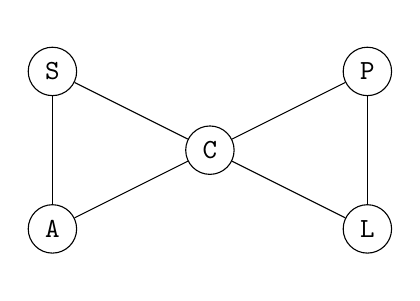
\begin{tikzpicture}			
            \tikzset{vertex/.style = {shape=circle, draw, minimum size=1.5em}}
			\tikzset{edge/.style = {- = latex'}}
			\tikzset{arrow/.style = {beamer_arrow, cdc_Blue}}
%			\tikzset{newRouting/.style = {thick, Red!70!black, dashed, ->,> = latex'}}
			\tikzset{newRouting/.style = {beamer_arrow, cdc_Green!70!black, dashed}}
			% vertices
%			\node[vertex, label={[align=left]below:\scriptsize{}Activity\\[-2mm]\scriptsize{}Center}] (u) at  (0,0)  {\texttt{A}};
%			\node[vertex, label={[align=left]above:\scriptsize{}Science and\\[-2mm]\scriptsize{}Technology}] (v) at  (0,2)  {\texttt{S}};
%			\node[vertex, label={[align=left]above:\scriptsize{}Central\\[-2mm]\scriptsize{}Office}] (x) at  (2,1){\texttt{C}};
%			\node[vertex, label={[align=left]below:\scriptsize{}Library}] (y) at  (4,0)  {\texttt{L}};
%			\node[vertex, label={[align=left]above:\scriptsize{}Post Office and\\[-2mm]\scriptsize{}Grocery Store}] (d) at  (4,2)  {\texttt{P}};

			\node[vertex, label={[align=left]below:\scriptsize{}}] (u) at  (0,0)  {\texttt{A}};
			\node[vertex, label={[align=left]above:\scriptsize{}}] (v) at  (0,2)  {\texttt{S}};
			\node[vertex, label={[align=left]above:\scriptsize{}}] (x) at  (2,1){\texttt{C}};
			\node[vertex, label={[align=left]below:\scriptsize{}}] (y) at  (4,0)  {\texttt{L}};
			\node[vertex, label={[align=left]above:\scriptsize{}}] (d) at  (4,2)  {\texttt{P}};

			%edges
        	\draw[edge] (v) to (u);
			\draw[edge] (v) to (x);
			\draw[edge] (u) to (x);
			\draw[edge, bend right=0] (y) to (d);
			\draw[edge] (y) to (x);
			\draw[edge] (d) to (x);
\end{tikzpicture}
	\subcaption{The connections of the example.}
		\label{fig:motivation_topology}
	\end{subfigure}%
~
	\begin{subfigure}[t]{0.49\textwidth}
		\centering
\begin{tikzpicture}			
            \tikzset{vertex/.style = {shape=circle, draw, minimum size=1.5em}}
			\tikzset{edge/.style = {- = latex'}}
			\tikzset{arrow/.style = {beamer_arrow, cdc_Blue}}
%			\tikzset{newRouting/.style = {thick, Red!70!black, dashed, ->,> = latex'}}
			\tikzset{newRouting/.style = {beamer_arrow, cdc_Green!70!black, dashed}}
			% vertices
%			\node[vertex, label={[align=left]below:\scriptsize{}Activity\\[-2mm]\scriptsize{}Center}] (u) at  (0,0)  {\texttt{A}};
%			\node[vertex, label={[align=left]above:\scriptsize{}Science and\\[-2mm]\scriptsize{}Technology}] (v) at  (0,2)  {\texttt{S}};
%			\node[vertex, label={[align=left]above:\scriptsize{}Central\\[-2mm]\scriptsize{}Office}] (x) at  (2,1){\texttt{C}};
%			\node[vertex, label={[align=left]below:\scriptsize{}Library}] (y) at  (4,0)  {\texttt{L}};
%			\node[vertex, label={[align=left]above:\scriptsize{}Post Office and\\[-2mm]\scriptsize{}Grocery Store}] (d) at  (4,2)  {\texttt{P}};
	
			\node[vertex, label={[align=left]below:\scriptsize{}}] (u) at  (0,0)  {\texttt{A}};
			\node[vertex, label={[align=left]above:\scriptsize{}}] (v) at  (0,2)  {\texttt{S}};
			\node[vertex, label={[align=left]above:\scriptsize{}}] (x) at  (2,1){\texttt{C}};
			\node[vertex, label={[align=left]below:\scriptsize{}}] (y) at  (4,0)  {\texttt{L}};
			\node[vertex, label={[align=left]above:\scriptsize{}}] (d) at  (4,2)  {\texttt{P}};



		
            % Routing 
      	\draw[arrow,->] (v) to (u);
		\draw[arrow,->] (u) to (x);
			\draw[arrow,->] (y) to (x);
		\draw[arrow,->] (x) to (d);
%            % Update
%        \only<4-5> {			\draw[newRouting] (v) to (x);}
%        \only<4> {			\draw[newRouting, bend right=20] (u) to (x);}
%        \only<4-8> {			\draw[newRouting] (y) to (d);}
%        \only<4-6,8-9> {			\draw[newRouting] (x.-55) to (y.180); }
%            % final
%%       \only<5->{			\draw[arrow, Red!70!black] (u) to (x);}
%%       \only<6->{        	\draw[arrow, Red!70!black] (v) to (x);}
%%       \only<7>{			\draw[arrow, Red!70!black] (x.-55) to (y.180);}
%%        \only<9-> {			\draw[arrow, Red!70!black] (y) to (d);}
%%        \only<10-> {			\draw[arrow, Red!70!black] (x) to (y);}
%       \only<5->{			\draw[arrow, cdc_Green!70!black] (u) to (x);}
%       \only<6->{        	\draw[arrow, cdc_Green!70!black] (v) to (x);}
%       \only<7>{			\draw[arrow, cdc_Green!70!black] (x.-55) to (y.180);}
%        \only<9-> {			\draw[arrow, cdc_Green!70!black] (y) to (d);}
%        \only<10-> {			\draw[arrow, cdc_Green!70!black] (x) to (y);}
%			% error
			
%		\only<7> { \node (error) at ($(x)!0.5!(y)$) {\Red\scalebox{2}{\LARGE \lightning}};}
\end{tikzpicture}
	\subcaption{The forwardings of the example.}
		\label{fig:initConf}
	\end{subfigure}%
	\caption{Example network topology and initial configuration of a software defined network. The corresponding input file
is given in Listing~\ref{lst:topology}.
%	\vspace{-0.25cm}
	}
	\label{fig:topology}
\end{figure}
The following grammar defines the input format.
%\vspace{-0.mm}
\begin{lstlisting}[captionpos=b, caption=Grammar of the topology and the initial configuration of SDNs., label = lst:grammar,language=ebnf]
ts			= name  description?  genOptions?  switches  cons
			  ingress  egress  forwarding EOF
name		= '.name' STR
description	= '.description' (STR | STR_MULTI)
genOptions  = '.options' (option (',' option)*)?

switches	= '.switches' switchT*
switchT		= sw (opts)?

opts		= '[' option (',' option)* ']'
option		= ID '=' STR

cons		= '.connections' con*
con			= sw sw (opts)?

sw			= ID | NAT

ingress     = '.ingress=' set
egress      = '.egress=' set

set         = '{' ( sw (',' sw)*) '}'

forwarding  = '.forwarding' forward*
forward     = sw '.fwd(' sw ')'

NAT         = '0'..'9'+
ID			= ('a'..'z'|'A'..'Z'|'_') ('a'..'z'|'A'..'Z'|'0'..'9'|'_')*

STR			= '"' ~('"' | '\n' | '\r' | '\t')*  '"'
STR_MULTI	= '"' ~('"' | '\t' )*  '"'
COMMENT		= ('//' ~('\n'|'\r')* | '/*' (. )*? '*/')
WS		    = ( ' ' | '\n' | '\r' | '\t')
\end{lstlisting}
%\vspace{-2.5mm}
Furthermore, \tool{} provides a parser for the concurrent overlapping updates.
%As an example of an concurrent update of the topology and initial configuration of Fig.~\ref{fig:topology}
%\texttt{upd(S.fwd(C)) || (upd(L.fwd(P)) >> upd(C.fwd(L)))}
%For more examples please see the updates in the example calls of Listing~\ref{lst:sdnEx}.
For examples please see the updates in the example calls of Listing~\ref{lst:sdnEx}.
\begin{lstlisting}[captionpos=b, caption=Grammar of the concurrent overlapping updates of SDNs., label = lst:grammar,language=ebnf]
result     	= update EOF
update      = swUpdate | seqUpdate | parUpdate

swUpdate    = 'upd(' idi '.fwd(' sidi ('/' idi)? '))'
seqUpdate   = '[' update (SEQ update)* ']'
parUpdate   = '[' update (PAR update)* ']'

sidi		= idi | '-'
idi 		= ID | INT

PAR 		= '||'
SEQ 		= '>>'

INT			= '0'..'9'+
ID  		= ('a'..'z'|'A'..'Z'|'_') ('a'..'z'|'A'..'Z'|'0'..'9'|'_')*

COMMENT		= ('//' ~('\n'|'\r')* | '/*' (. )*? '*/')
WS			= ( ' ' | '\n' | '\r' | '\t')
\end{lstlisting}

\subsection{LTL and Flow-LTL}
\tool{} also provides a parser for the temporal logics LTL and Flow-LTL. 
For examples please see the example calls of \tool{} of Listing~\ref{lst:pnLTLEx} and Listing~\ref{lst:pnwtFlow-LTLEx}.
The syntax is given by the following grammar.
\begin{lstlisting}[captionpos=b, caption=Grammar of the temporal logics Flow-LTL, label = lst:grammar,language=ebnf]
flowLTL 		= runFormula EOF

runFormula 		= ltl | '(' ltl rimp runFormula ')' | runBinary | flowFormula
runBinary 		= '(' runFormula rbin runFormula ')'
flowFormula 	= forallFlows ltl

ltl 			= ltlUnary | ltlBinary | tt | ff | atom
ltlUnary 		= unaryOp ltl
ltlBinary 		= '(' ltl binaryOp ltl ')'

atom 			= ID | INT

// LTL
unaryOp 		= (ltlFinally | globally | next | neg)
binaryOp 		= (and | or | imp | bimp | until | weak | release )
ltlFinally 		= 'F'
globally 		= 'G'
next 			= 'X'
neg 			= 'NEG' | '!'
and 			= 'AND'
or 				= 'OR' 
imp				= 'IMP' | '->'
bimp			= 'BIMP' | '<->'
until 			= 'U'
weak 			= 'W'
release 		= 'R'

// FlowFormula
forallFlows 	= 'A'

// RunFormula
rbin 			= rand | ror
rand 			= 'AND'
ror				= 'OR'
rimp 			= 'IMP' | '->'

tt 				= 'TRUE'
ff 				= 'FALSE'

INT 			= '0'..'9'+
ID  			= ('a'..'z'|'A'..'Z'|'_') ('a'..'z'|'A'..'Z'|'0'..'9'|'_')*

COMMENT			= ('//' ~('\n'|'\r')* | '/*' (. )*? '*/')
WS				= ( ' ' | '\n' | '\r' | '\t')
\end{lstlisting}
%\section{The Output Formats}


\chapter{Contact}
We appreciate your feedback on \tool{}. Please send any bugs, comments, or
questions to:
\begin{center}
 manuel.gieseking(at)informatik.uni-oldenburg.de
\end{center}
%Have fun using \tool{}!

%%%%%%%%%%%%%%%%%%%%%%%%%%%%%%%%%%%%%%%%%%%%%%%%%%%%%%%%%%%%%%%%%%%%%%%%%%%%%%%
\appendix
\chapter{Detailed List of Modules and Parameters}
\label{app:detailedModules}
In the following we list the help dialogues of each module.
That is, how to call the module, the possible 
and needed parameters including their explanations.
\begin{subappendices}
\subimport{./dialogs/}{helpDialogs}
\end{subappendices}
\end{document}
